\chapter{Domande per Prepararsi per l'Esame}

\section{PROLOG}

\qs{}{Scrivere un semplice programma PROLOG che va in loop.}


\begin{figure}[h]
    \centering
    \begin{minipage}{0.45\textwidth}
        \centering
        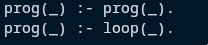
\includegraphics[scale=0.5]{Domande/loop1.png}
        \caption{Codice che causa un loop.}
    \end{minipage}
    \hfill
    \begin{minipage}{0.45\textwidth}
        \centering
        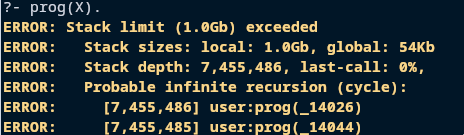
\includegraphics[scale=0.35]{Domande/loop2.png}
        \caption{PROLOG se ne accorge perché è un loop stupido.}
    \end{minipage}
\end{figure}


\qs{}{Fare l'esempio del pinguino.}

\begin{figure}[h]
    \centering
    \begin{minipage}{0.45\textwidth}
        \centering
        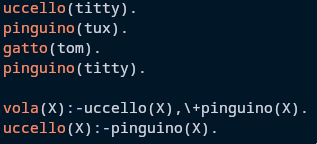
\includegraphics[scale=0.5]{Domande/pinguino1.png}
        \caption{Codice dell'esempio.}
    \end{minipage}
    \hfill
    \begin{minipage}{0.45\textwidth}
        \centering
        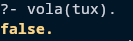
\includegraphics[scale=0.65]{Domande/pinguino2.png}
        \caption{Tux è un pinguino, quindi non vola (negazione per fallimento).}
    \end{minipage}
\end{figure}



\qs{}{Perché in PROLOG non è presente la negazione forte (negazione classica)?}

\paragraph{Risposta:} perché in prolog si assume mondo chiuso e ragionamento non monotono. La negazione classica richiede la conoscenza completa del dominio per poter affermare che qualcosa sia vero o falso, ma in prolog si possono aggiungere nuovi fatti.

\qs{}{Come funziona la negazione per fallimento?}

\paragraph{Risposta:} semplicemente un determinato \\+P è vero se prolog non riesce a dimostrare P. In poche parole "se non sono in grado di dimostrare che un qualcosa sia vero allora il suo opposto è vero".

\qs{}{Fare un esempio di negazione per fallimento.}

\nt{Andare a vedere l'esempio del pinguino.}

\qs{}{Tipi di fallimenti in PROLOG.}

\paragraph{Risposta:}

\begin{itemize}
  \item Successo se $G_n$ è vuoto (\texttt{true}). 
  \item Fallimento finito, se non è possibile derivare da $G_n$ alcun risolvente e $G_n$ non è vuoto (\texttt{false}).
  \item Fallimento infinito, se è sempre possibile derivare nuovi risolventi (loop infinito).
\end{itemize}

\qs{}{Che cos'è la logica monotona?}

\paragraph{Risposta:} una logica dello stesso tipo della logica classica, in cui si ha una conoscenza completa e non si aggiungono o rimuovono nuovi fatti.

\qs{}{Come funziona la ricerca SLD?}

\paragraph{Risposta:} la ricerca SLD è l'algoritmo inferenziale usato da prolog per risolvere obiettivi. Andare a vedere l'algoritmo di costruzione dell'albero SLD.

\nt{Nota per self: è SDL, non LSD.}

\qs{}{Perché si usa la risoluzione SLD se è completa solo con le clausole di Horn?}

\paragraph{Risposta:} per questioni di efficienza, inoltre prolog usa solo clausole di Horn, quindi non è un dramma. 

\qs{}{Spiegare il cut(!) e qual è il suo vantaggio.}

\paragraph{Risposta:} il cut è un predicato extra logico che consente di modificare l'esecuzione dell'interprete PROLOG (è un predicato sempre vero). Il suo vantaggio è che blocca il backtracking rendendo definitive le scelte fatte. Questo fa perdere la completezza, ma aumenta l'efficienza evitando di esplorare rami potenzialmente inutili.

\qs{}{Scrivere un programmino con il cut(!).}

\begin{figure}[h]
    \centering
    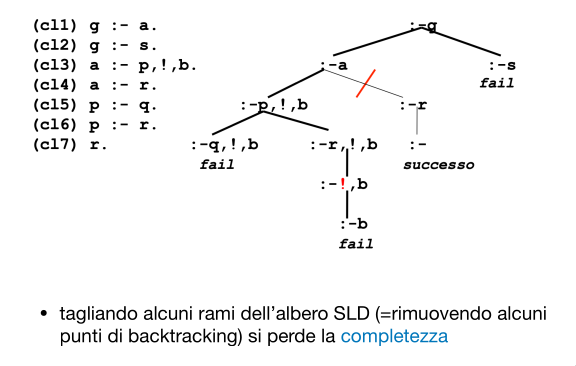
\includegraphics[scale=0.2]{Domande/cut.png}
    \caption{Esempio di programma con il cut.}
\end{figure}

\paragraph{Risposta:}

\qs{}{Cut(!) danneggia la correttezza o la completezza? Perché?}

\paragraph{Risposta:} la completezza, perché va a escludere potenziali soluzioni che sarebbero state considerate facendo backtracking.

\qs{}{Scrivere lo stack dell'interprete PROLOG di un codice in cui è presente il cut(!).}

\section{ASP}

\qs{}{Dire se un dato programma è PROLOG o ASP.}

\nt{Suggerimento: guardare se il programma ha cut (PROLOG) o no (ASP)}

\qs{}{Differenze tra PROLOG e CLINGO.}

\paragraph{Risposta:}

\begin{itemize}
  \item ASP (CLINGO) ha integrity constrain, PROLOG no.
  \item ASP è proposizionale, PROLOG è logica del primordine. 
\item In ASP l’ordine dei letterali non ha alcuna importanza. 
  \item Prolog è goal-directed, ASP no.
  \item In ASP non c'è il concetto di dimostrazione.
  \item La SLD-risoluzione del Prolog può portare a loop,
mentre gli ASP solver non lo consentono (aka. ASP non va in loop). 
\item PROLOG ha il cut(!), ASP no.
\item ASP ha sia la negazione per fallimento che la negazione classica, PROLOG solo la negazione per fallimento.
\end{itemize}

\qs{}{Esempio di Nixon pacifista.}

\begin{figure}[h]
    \centering
    \begin{minipage}{0.45\textwidth}
        \centering
        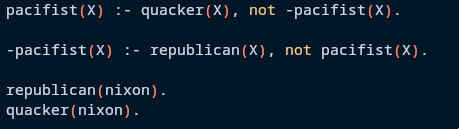
\includegraphics[scale=0.5]{Domande/nixon1.png}
        \caption{Codice di Nixon pacifista.}
    \end{minipage}
    \hfill
    \begin{minipage}{0.45\textwidth}
        \centering
        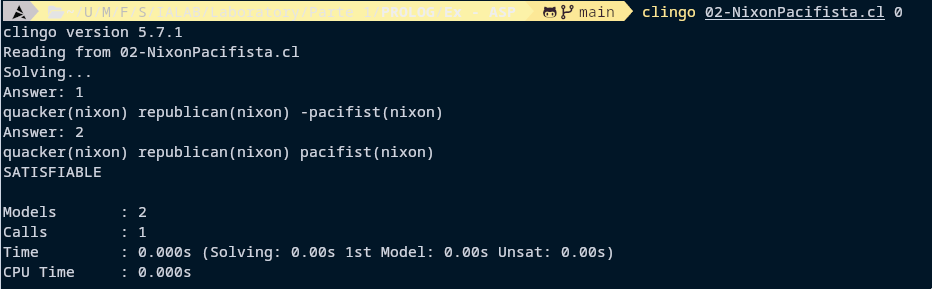
\includegraphics[scale=0.25]{Domande/nixon2.png}
        \caption{Modelli di Nixon pacifista.}
    \end{minipage}
\end{figure}


\qs{}{PROLOG e ASP sono monotoni?}

\paragraph{Risposta:} non lo sono perché è possibile aggiungere nuovi fatti e quindi non si ha la completa conoscenza del dominio.

\qs{}{Perché in ASP non c'è il cut(!)?}

\paragraph{Risposta:} non esistono né una dimostrazione né backtracking, ASP si cerca i suoi modelli indipendentemente.

\qs{}{Come funziona la negazione per fallimento in ASP?}

\paragraph{Risposta:} un determinato "not a" è vero se e solo se "a" non è dimostrabile in un answer set. Ciò che non può essere derivato è considerato vero.

\qs{}{Che cos'è l'Integrity Constrain e a cosa serve?}

\paragraph{Risposta:} è una regola senza testa (:- something). Serve a vietare che certe combinazioni di fatti siano presenti nello stesso answer set. Se il corpo è vero in un modello $X$ allora quel modello viene scartato. Serve per "filtrare" gli insiemi di risposta validi.

\qs{}{In PROLOG si può avere Integrity Constrain?}

\paragraph{Risposta:} non sono nativi, ma è possibile simularli utilizzando la negazione per fallimento. 

\qs{}{Fare un esempio di codice ASP che risulta insoddisfacibile.}

\begin{figure}[h]
    \centering
    \begin{minipage}{0.45\textwidth}
        \centering
        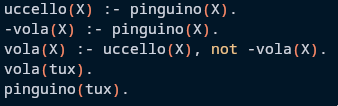
\includegraphics[scale=0.5]{Domande/tux1.png}
        \caption{In questo esempio si ha che tux vola ma non vola.}
    \end{minipage}
    \hfill
    \begin{minipage}{0.45\textwidth}
        \centering
        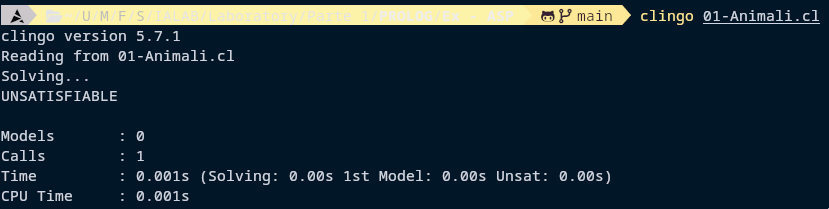
\includegraphics[scale=0.25]{Domande/tux2.png}
        \caption{Non esistono modelli che siano vero.}
    \end{minipage}
\end{figure}


\qs{}{Come modificare un semplice programma ASP per renderlo soddisfacibile.}

\nt{Suggerimento: rimuovere le contraddizioni.}

\qs{}{Che cos'è e a che cosa serve il ridotto di un programma?}

\dfn{Ridotto}{
  Il \newfancyglitter{ridotto} $P^S$ rispetto a un insieme di atomi S: 
  \begin{itemize}
    \item Rimuove ogni regola il cui corpo contiene $not L$, per $L \in S$. 
    \item Rimuove tutti i $not L$ dai corpi delle restanti regole.
  \end{itemize}

  $P^S$ non contiene atomi con negazione per fallimento: 
  \begin{itemize}
    \item Ha un unico answer set. 
    \item Se tale answer ser coincide con S, allora S è un answer set per P.
  \end{itemize}
}

\qs{}{Fare il ridotto di un programma ASP rispetto a un insieme dato.}

\begin{center}
  p :- a.

a :- not b.

b :- not a.
\end{center}

\nt{In questo esempio il ridotto c'è per S = \{b\} e S = \{a, p\}}

\qs{}{Dire se un programma ASP presenta un answer set.}

\paragraph{Risposta:}

\qs{}{Scrivere un programma che presenti due answer set diversi.}

\paragraph{Risposta:} banalmente si può scrivere il programma di Nixon pacifista. Ha un answer set in cui Nixon è pacifista e quacchero e un answer set in cui Nixon è repubblicano e guerrafondaio (non pacifista).

